%%
%% This is file `./samples/longsample.tex',
%% generated with the docstrip utility.
%%
%% The original source files were:
%%
%% apa7.dtx  (with options: `longsample')
%% ----------------------------------------------------------------------
%% 
%% apa7 - A LaTeX class for formatting documents in compliance with the
%% American Psychological Association's Publication Manual, 7th edition
%% 
%% Copyright (C) 2019 by Daniel A. Weiss <daniel.weiss.led at gmail.com>
%% 
%% This work may be distributed and/or modified under the
%% conditions of the LaTeX Project Public License (LPPL), either
%% version 1.3c of this license or (at your option) any later
%% version.  The latest version of this license is in the file:
%% 
%% http://www.latex-project.org/lppl.txt
%% 
%% Users may freely modify these files without permission, as long as the
%% copyright line and this statement are maintained intact.
%% 
%% This work is not endorsed by, affiliated with, or probably even known
%% by, the American Psychological Association.
%% 
%% ----------------------------------------------------------------------
%% 
\documentclass[man]{apa7}
% \documentclass[man, mask, floatsintext]{apa7}

\usepackage[american]{babel}
\usepackage{nicefrac}
\usepackage{todonotes}
\usepackage{epigraph}
\usepackage{amsfonts, amsmath,amssymb}

\newcommand{\SR}[1]{} %for EJ's bibtex file
\newcommand{\given}{\, | \,}
\newcommand{\EJ}[1]{\todo[inline, color=green]{  #1 }}
\newcommand{\JR}[1]{\todo[inline, color=gray]{  #1 }}
\newcommand{\MK}[1]{\todo[inline, color=red]{  #1 }}

\usepackage{graphicx}
\graphicspath{ {images/} }

\usepackage{csquotes}
\usepackage[style=apa,sortcites=true,sorting=nyt,backend=biber]{biblatex}
\DeclareLanguageMapping{american}{american-apa}
\addbibresource{bibliography.bib}
\addbibresource{referenties.bib}

% \setlength{\parindent}{8ex}

% \usepackage{authblk}

\title{Building Trust in Science Through a Bayesian Perspective on Probability and Uncertainty}
\shorttitle{Building Trust Through a Bayesian Perspective}

\threeauthors{Joshua M. Rosenberg}{Marcus Kubsch}{Eric-Jan Wagenmakers}
\threeaffiliations{University of Tennessee, Knoxville}{IPN - Leibniz Institute for Science and Mathematics Education}{University of Amsterdam}

% \authorsnames[1,2,3]{Joshua M. Rosenberg, Marcus Kubsch, Eric-Jan Wagenmakers}
% \authorsaffiliations{{University of Tennessee, Knoxville},{IPN - Leibniz Institute for Science and Mathematics Education},{University of Amsterdam}}

\leftheader{Weiss}

\abstract{
Uncertainty is ubiquitous in science, but scientific understanding is often represented to the public and in educational contexts as certain and immutable. Adding to this problem is that when scientists try to communicate their uncertainty, research has demonstrated that many people--learners and experts alike--struggle to interpret the statistics that are often used to make inferences about evidence from scientific data. We conjecture that a Bayesian perspective can offer a foundation for teaching and learning about a persistent but sometimes unsettling tension for science, making sense of and communicating about uncertainty. Central to this approach is viewing uncertainty \ital{probabilistically}, as doing so provides a language for expressing the degree of uncertainty in knowledge across a range of scientific domains and socio-scientific issues. In this paper, we elaborate on the importance of probability and uncertainty in science (and science education) and review how people learn about these concepts---and when and why they face difficulties when doing so. Then, we provide an accessible primer on Bayes Theorem and more general principles following from the application of Bayes Theorem. Next, we provide examples of how a Bayesian perspective could inform efforts around both science literacy and science education with an emphasis upon building trust in science. We conclude with directions for future research focused on bolstering trust in science outside of and within pre-collegiate science classrooms, where a Bayesian perspective can provide a coherent approach to engaging in science to make sense of scientific ideas in a principled yet flexible manner.
}

\keywords{Bayesian, uncertainty, probability, trustworthiness, statistics}

\authornote{
   \addORCIDlink{Joshua M. Rosenberg}{0000-0003-2170-0447}
   \addORCIDlink{Marcus Kubsch}{0000-0001-5497-8336}
   \addORCIDlink{Eric-Jan Wagenmakers}{0000-0003-1596-1034} 
   \\
   Joshua M. Rosenberg and Marcus Kubsch contributed equally to this manuscript.
}

\begin{document}
\maketitle

\setlength{\epigraphwidth}{1.0\textwidth} % set for individual epigraph
\epigraph{It is seen in this essay that the theory of probabilities is at bottom only common sense reduced to calculus; it makes us appreciate with exactitute that which exact minds feel by a sort of instinct without being able ofttimes to give a reason for it . . . we shall see that there is no science more worthy of our meditations, and that no more useful one could be incorporated in the system of public instruction.}{Pierre-Simon Laplace, 1829}
\setlength{\epigraphwidth}{0.4\textwidth} % return to default for the next epigraphs
%\nocite{Laplace18291902} %[p. 196]

Uncertainty is ubiquitous in science and creating ways to account for this uncertainty has helped science to progress. Consider, for instance, uncertainty due to the measurements or instruments used to study phenomena: In such cases, error due to measurement can be incorporated into models through the repeated measures of the same object or phenomenon \parencite{pls03}. Measurement is also present when the object that is measured--like a plant--is variable in its characteristics because of environmental and genetic variation (and interactions among these sources of variation) between the individual plants \parencite{pls03}. Another form of uncertainty is accounted for in terms of its central role within explanatory theories--such as those associated with evolution and quantum physics--for which models take the form of probabilistic statements about the world \parencite{g00}. 

Negotiating the many forms of uncertainty through (constructively) arguing—-and building toward consensus at the same time that uncertainty is present—-is a key part of the scientific process \parencite{duschl2008science, t00, nrc12}. Concomitantly, some philosophers of science have suggested that science is a process that builds increasingly better models which allows us to make increasingly more accurate predictions \parencite{g10, g06, n02, r77}. However, while scientists and historians and philosophers of science are well aware of the uncertainty (and limitations) around scientific knowledge and the practice of negotiating and arguing from evidence, scientific knowledge is often represented to the public and in educational contexts as certain and immutable \parencite{d90}. Trust in science can erode and has eroded when scientists individually or collectively change their views, such as during the first phase of the COVID-19 crisis, when scientists faced serious criticism from the public, the media, and elected representatives for changing their recommendations based upon new scientific data and findings. A similar tension is now present concerning vaccines for COVID-19--a tension that involves reconciling robust but still initial clinical trial data and new data from population-level vaccination efforts and making policy-level recommendations (and individual decisions) amid this uncertainty.
Adding to this difficult state of affairs regarding the role of uncertainty in science is that when scientists try to communicate their uncertainty, prior research has demonstrated that many people–learners and experts alike–struggle to interpret the statistics and derivations of statistics (such as standard errors/margins of error and confidence intervals) and that are often used to make inferences from scientific data \parencite{gkv04, s07, tk74}. Similarly, difficulties in understanding the technical language of probability can contribute to a struggle on the part of students when learning about concepts such as evolution and nuclear decay that are modeled in terms of probabilistic statements \parencite{fth17}.

In this paper, we argue that these challenges concerning trust in scientific knowledge that not only can but must change can be addressed in a principled, flexible way, but that doing so requires making use of a Bayesian perspective that heretofore has been under-used outside of particular scientific and engineering domains---domains that often make little contact with science educators and researchers with an interest in building trust in science. Yet, the opportunity to do so now exists for technical and social reasons. Based on accumulating evidence from psychologists using Bayesian models of cognition \parencite{g12, tgk06}, statisticians and statistics educators advancing tools and practices for Bayesian methods \parencite{a02, b02, h_a20, h_j20,me14, s07} and science education scholars who have advanced a Bayesian perspective on argumentation \parencite{n11, s07}, we conjecture that a Bayesian perspective can help people--and science learners--to understand and reason about uncertainty in a way that leverages their existing ways of thinking. Central to this conceptualization is viewing uncertainty \ital{probabilistically}, as probabilities can provide a language for expressing the degree of uncertainty in our knowledge in a wide range of domains \parencite{g12}. In drawing on research from psychologists, learning scientists, and educational researchers, we make this conjecture not only on the merits of Bayes' Theorem as a mathematical or statistical tool, but primarily on evidence that the perspective we are advocating can provide an intuitive way for people to think about data and evidence in the world \parencite{g12} and in classroom contexts \parencite{ll20, n11, s07, so12, w17}.

\section{Uncertainty in Science and the Central Role of Probability}

Probability and uncertainty are ubiquitous in scientific methodologies, scientific concepts, and in how science is communicated \textcite{gsoobmc17}. The practice of science often begins with measurement for which measurement error--which has a random component--is endemic. This random component arises from random variations in the measurement process and limits the certainty that one can have in the measurements. Reducing that measurement error has been critical for many discoveries in science, such as in sorting out the periodic table as we know it today \parencite{fco15}. However, deciding on adequate statistical procedures to determine measurement uncertainty regularly sparks debate, e.g., the recent study on the relationship between SARS-CoV-2 viral load and patient age by \textcite{jmvbzhd20} was heavily debated in the scientific community \parencite{frick_peer-review_2020}.

Probability and uncertainty are not only key concepts in science practices (such as analyzing and interpreting data) but are also an integral part of explanatory models of and theories for scientific concepts. For example, in the context of Heisenberg’s uncertainty principle and--more generally--quantum mechanics \parencite{feynman1951operator}, confidence is limited not only by measurement error but in principle---even in the perfect experimental setup there is no deterministic outcome. Instead, one has to calculate the probability of each possible outcome using the Born rule. 
To this day, there is an ongoing argument among physicists and philosophers about how to interpret probability and the puzzling quantum mechanical phenomena such as quantum tunneling \parencite{c19}. Another example of how probability and uncertainty are central to learning scientific concepts is evolution \parencite{fsnh19}. Evolution is modeled as a probabilistic process as the emergence of new variations (e.g., through mutations) can only be described probabilistically. Further, the continued survival of these variations is governed by phenomena such as natural selection or random drift which also escape a deterministic description and are thus modeled probabilistically. Similar to within quantum physics, how to interpret this probability has also sparked debate among researchers \parencite{m16}. 
Given that probability and uncertainty spark debate among scientists, it is perhaps unsurprising that misinterpretations happen when scientists in the natural and engineering sciences communicate about their findings with their peers or the public \parencite[]{gkv04, c14, mg17}. For example, error bars in the form of confidence intervals are routinely interpreted as distributions that assign a higher probability to the center of the interval \parencite{kl18} or \emph{p}-values are interpreted as effect sizes \parencite{gc17, n14} (although p-values describe how (in)compatible a set of data is with a set of assumptions. In sum, misinterpretations of statements about probability and uncertainty are common across the range of modes in which scientists communicate about their work.

\section{Uncertainty in Science Education}

\subsection{The Roles of Probability Across Scientific Disciplines}

Given the above-noted roles of probability in scientific concepts and theories, it is unsurprising that educational researchers have documented how students learn about probability. As one example, probability and chance events play an important role in the life sciences \parencite{g03, gk08}, particularly in evolutionary processes and learning about them \parencite{th17}. Recently, \textcite{fsnh19} investigated the relation between statistical reasoning and acceptance and knowledge about evolution in a large sample of nearly 500 university students in the US. They found that students’ statistical reasoning capabilities are a strong predictor of both acceptance of evolution and knowledge about evolution.  

In the physical sciences, students' struggles with the probabilistic nature of quantum physics \parencite{br02} and nuclear decay \parencite{smmv17} have been established, but the underlying reasons and mechanisms remain less researched than in evolution. Research into students’ misconceptions inspired by conceptual change research has started to address this gap \parencite{ms15, alra14, st09}. Findings mirror the position of \textcite{bgv94}. Specifically, the concepts of probability are taught abstractly and in such a way that does not build upon the ideas that students already hold, the experiences that students have, and the language that students use. Thus, these studies affirm students' struggles with scientific concepts that are probabilistic but hint at an underlying issue of more foundational challenges with reasoning about probability beyond science education contexts. 

Indeed, past research has shown that the language and representations used to communicate probability and uncertainty independent of specific scientific content domains or scientific practices are also known to present difficulties to learners. The work of \textcite{tk74}, especially, points to a whole range of biases that the language in which statements about probability and uncertainty are framed can elicit. A prominent example is the neglect of base rate information in the (timely) context of medical testing, that is, the probability of having a medical condition based on a positive test result is often hugely overestimated because information about the base rate of people affected from the condition is neglected \parencite{kahneman_thinking_2012}.

Responding to and building upon Kahneman and Tversky's work, Gigerenzer and colleagues provided important insights into the underlying mechanisms for the occurrence of these biases. Their research suggests that the biases are at least partly the result of information about probability and uncertainty being provided in a way that is incompatible with the heuristics that people develop from their everyday experiences \parencite{gh95, jkg18}. Based upon this premise, \textcite{jkg18} were able to demonstrate that students judge probability significantly better when language is adopted that better aligns with the heuristics that most learners develop from their everyday experiences. In sum, it seems feasible to change representations of probability and uncertainty so that they better align with ideas and heuristics that learners hold so that these support, rather than hinder, learning.

\subsection{Uncertainty in the Context of Analyzing and Interpreting Data}

Recent work--primarily by developmental psychologists and scientists--has applied Bayesian ideas to a new context: how children make sense of and world \parencite{g12, tgk06, tgk06}. This notion that children reason about the world in a way that is analogous to Bayes Theorem is in some ways surprising, but it also builds upon much earlier work that also documented the surprisingly complex ways that children could reason about the world---as well as the assumed limitations of children's reasoning, the work of \textcite{pi69}. Different from earlier work on the stages through which children develop, recent work using Bayesian models considers the differences in the reasoning ability of children and adults to be a matter of degree, rather than kind. In short, children hold initial ideas and understandings that they change (or update) in ways that are concordant with how Bayes Theorem represents the updating of an initial belief in light of data (and how the Bayesian Learning Cycle described earlier allows individuals to integrate inductive and deductive reasoning).

In addition to developmental research that uses Bayes Theorem as an analog for how children make sense of data and information in light of their initial ideas and beliefs, other work bears a striking semblance to developmental research that does. In particular, research on how learners’ prior understanding influence how they make sense of how likely different patterns in data are centers the same tension around interpreting data in light of initial beliefs that a Bayesian perspective highlights \parencite[e.g., ][]{kd88, mkm07, ssc07}. While these studies have focused on how students’ prior ideas and data interact, Bayesian frameworks were not used to formalize this process of integrating data.

A Bayesian view of how children learn from their experiences and update their beliefs about the world has become especially prominent over the past 10-15 years \parencite{gt07, gw12}. Because of this, one might assume that there has been a ready application of these ideas about how children think about the world in a Bayesian way to education and developmental scientists have pointed to this opportunity. For instance, \textcite{g12} wrote that the use of Bayesian methods to understand child development can serve as “a scientific foundation for a long tradition on ‘inquiry-based’ science education,” that “could lead us to much more specific and scientifically supported proposals for education” (p. 1627). 

However, despite arguments such as Gopnik's (2012) for integrating developmental and educational research, it has largely not been the case that “science itself could help turn young children’s natural curiosity and brilliance into better science teaching and learning” \textcite[p. 1627]{g12}, as some science education scholars have bemoaned \parencite{ls15}). Indeed, scholars have argued that it is often obsolete applications of Piaget’s ideas \parencite[e.g., ][]{pi69} that represent the greatest contribution of developmental ideas to education \textcite{ls07}. We argue that this is still largely the case in the present, despite advances in both developmental research as well as statistical methodology related to Bayesian ideas—and that it is time to start exploring how bringing out the inherent Bayesian ways of thinking in education may provide support for learners’ efforts to make sense of the world.

At the same time that opportunities to connect developmental science with education (especially science education), science education research has emphasized how important students' prior knowledge and understandings are to their understanding of scientific concepts and processes \parencite[e.g., ][]{ssc07}. For example, \textcite{mkm07} summarized findings across several studies showing that when elementary grade students reasoned with data in a context about which they had strong and valid prior understandings that informed their interpretation of data (about force and motion in the context of ramps), and they were able to explain sources of error in the data \parencite{mk03}, but when the data was in a context they did not understand well, they struggled to distinguish between random variation due to sources of error and sources of variation due to something that was causing a difference in the data (generated by measuring the motion of pendulums). Later design- and laboratory-based research has shown that students can develop an understanding of scientific ideas through the analysis of data \parencite{ls04,mkk17}.

In summary, developmental and psychological research into Bayesian models of cognition supports and bolsters efforts in education--especially science education--to design instruction based around eliciting and understanding students’ ideas \parencite{gb16, hbavb20, wtbs12}. There is an opportunity to use Bayesian ideas as a framework for formalizing these ideas about how prior ideas affect students’ reasoning about data and how teachers can leverage students’ ideas to design instruction, but a Bayesian perspective has--with a few exceptions focusing on how Bayes Theorem can provide a model for the science practice of argumentation \parencite[e.g., ][]{n11, so12}--has been absent from research in science education.

After having reviewed how people learn about probability and uncertainty and where they face difficulties and research on uncertainty in the context of analyzing data, we next formally introduce Bayes Theorem and describe the broader process through which one's beliefs can be revised, or updated, in a way that leverages both inductive reasoning from data and deductive reasoning from beliefs or principles--what we refer to as the \ital{Bayesian Learning Cycle}. We also describe some of the ways of knowing, or epistemological considerations, that follow from Bayes Theorem and which comprise a core part of the Bayesian perspective that we argue has a role in building trust in science.

\section{A Primer on Bayes Theorem and a Bayesian Epistemology}

\subsection{An Accessible Introduction to Bayes Theorem}

At its core, Bayes' theorem provides a means to update one's beliefs about the world from observations in such a way that prior knowledge can be used in a principled manner. As represented in Equation 1, Bayes' Theorem states that at any point in time, our knowledge about the world after making a new observation (i.e., our posterior knowledge) can be obtained by multiplying our prior knowledge with a predictive updating factor (e.g., \cite{RouderMorey2019,WagenmakersEtAl2016CD} ):
\begin{equation*}
        \text{Posterior uncertainty} = \text{Prior uncertainty} \times \text{Predictive updating factor}.
\end{equation*}
Mathematically, this can be expressed as  
\begin{equation}
\label{eq:BayesRule}
        p(\theta \mid \text{data}) = p(\theta) \times \frac{p(\text{data} \mid \theta)}{p(\text{data})},
\end{equation}
where $\theta$ is a hypothesis, proposition, claim, parameter value, or in general any particular account of the world about which we are uncertain. The predictive updating factor consists of two components. First, $p(\text{data} \given \theta)$ is the likelihood, that is, the extent to which the observed data were expected under $\theta$. Second, $p(\text{data}$ is the marginal likelihood, that is, the extent to which the observed data were expected without conditioning on $\theta$. If the observed data are more expected (i.e., better predicted) when conditioning on $\theta$, the predictive updating factor is higher than 1, and $\theta$ becomes more credible. 

To illustrate the above equation, consider the following: An educator is interested in the proportion of students that use Windows or MacOS as their operating system. The proportion of Windows users $\theta$ ranges between 0 and 1. Before you start our Bayesian analysis, you need to quantify your background knowledge -- the relative plausibility of the different values for $\theta$. Given their previous experiences as a teacher, their best guess is that about half of the students use Windows. They would not be surprised if the proportion of Windows users was between 30\% and 70\% but you would be rather surprised to find either no Windows or exclusive Windows usage. 

This background knowledge motivates the use of the dome-shaped prior distribution shown as the dashed line in Figure~\ref{fig:WindowsMacPriorPosterior}.\footnote{This is the beta$(2,2)$ distribution.} Now suppose you start to collect data by asking students about the operating systems of their computers. The first ten observations of Windows (W) and MacOS (M) usage that you make are $\{W, W, M, W, M, W, W, M, W, M\}$: six students use Windows and four use MacOS. 

With these data in hand, we then combine our prior knowledge (i.e., the dome-shaped prior distribution) with the predictive updating factor (assuming a binomial likelihood) and obtain the posterior distribution shown as the solid line in Figure~\ref{fig:WindowsMacPriorPosterior}. The posterior distribution is more peaked than the prior distribution, indicating that the data have sharpened our knowledge about $\theta$. In addition, the posterior distribution is higher than the prior distribution for values of $\theta$ between approximately $.4$ and $.75$: these values of $\theta$ predicted the data relatively well and have therefore gained credibility. In contrast, values of $\theta$ lower than $.4$ and higher than $.75$ predicted the data relatively poorly, which is why they have lost credibility compared to the prior.\footnote{Note that the area under a probability distribution equals 1, so that posterior gains for specific regions of $\theta$ cancel out exactly against posterior losses for the other regions.} 

\begin{figure*}[h]
\begin{center}
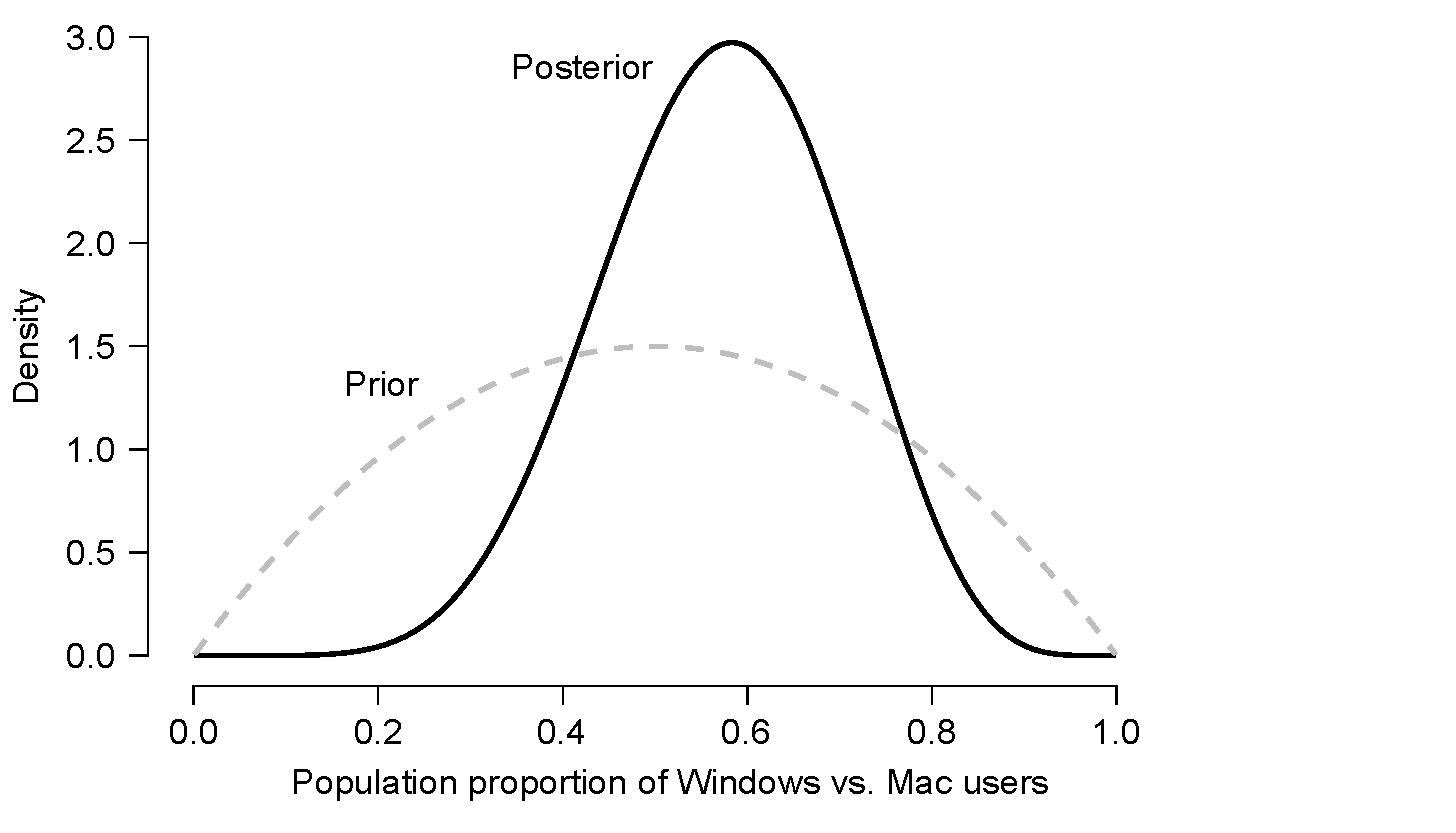
\includegraphics[width = .785\paperwidth]{WindowsMacPriorPosterior.pdf}
\caption{Simple example of Bayesian learning. A dome-shaped prior distribution captures the background knowledge concerning the proportion of students using Windows vs. MacOS. Observing fictitious data from 10 students (six using Windows, four using MacOS) drives a knowledge update that results in a bell-shaped posterior distribution. Figure based on the \emph{Learn Bayes} module in JASP.}
\label{fig:WindowsMacPriorPosterior}
\end{center}
\end{figure*}

Although we demonstrated this updating process in a single step, it could also be executed sequentially, one student at a time. For instance, the first observation you make is a $W$ and in light of your prior this makes Windows usage a little more likely than MacOS usage. This slight change in knowledge is reflected in the difference between the distributions on the top two lines in Figure~\ref{fig:WindowsMacSequential}; line ``0'' represents the dome-shaped prior distribution and line ``1'' represents the posterior distribution after the first observations. Note that observing a $W$ has nudged the distribution a little to the right. Crucially, the `nudged' posterior distribution after the first observation now takes the role of the prior distribution ready to be updated by our second observation. The second observation is again a $W$, and line ``2'' shows that the resulting posterior distribution is nudged to the right once more. At every stage in the sequential updating process, the posterior distribution based on the observations seen so far becomes the prior distribution for incorporating the information from the next observation. Specifically, the changing distributions in Figure~\ref{fig:WindowsMacSequential} show our knowledge about the world is subject to constant change, by making observations and integrating incoming information with current knowledge using Bayes' theorem. It should be emphasized that although the updating process is conceptually different, the final outcome is identical: the shape of the posterior distribution is unaffected by whether data arrive simultaneously or sequentially.

\begin{figure*}[h]
\begin{center}
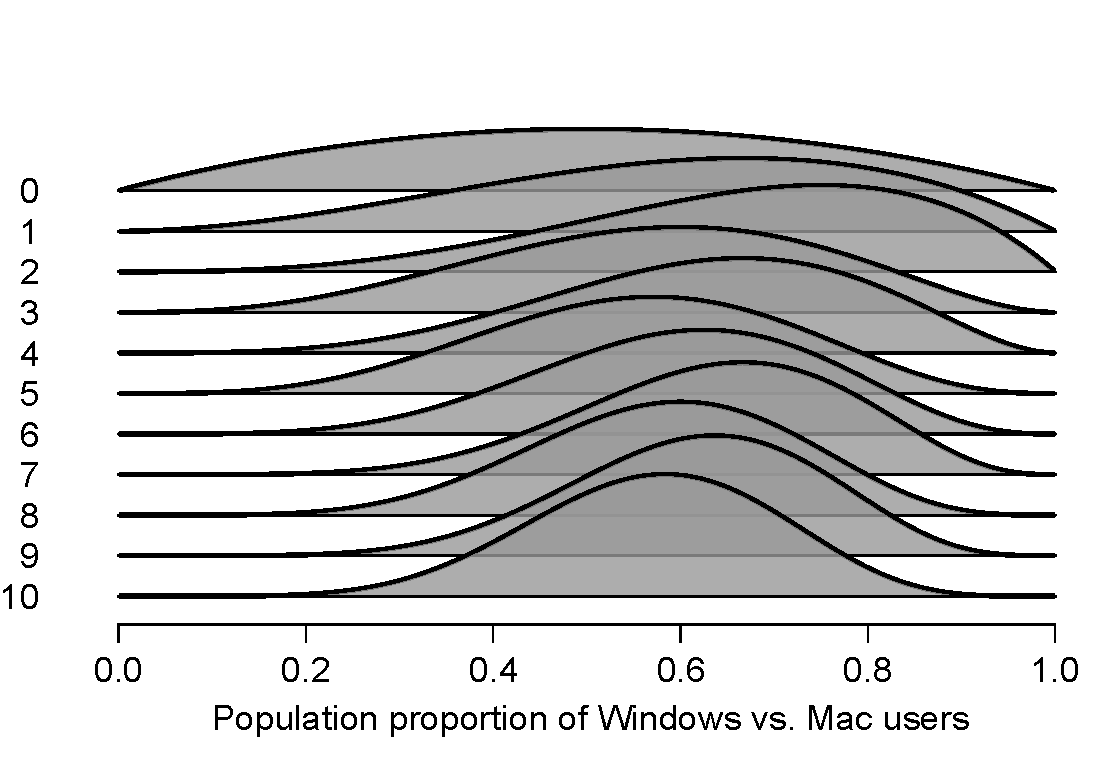
\includegraphics[width = .65\paperwidth]{WindowsMacSequential.pdf}
\caption{Sequential Bayesian learning. A dome-shaped prior distribution (line ``0'') captures the background knowledge concerning the proportion of students using Windows vs. MacOS. Each new observation results in an update to a posterior distribution, which then becomes the prior distribution for the analysis of the next observation. Figure based on the \emph{Learn Bayes} module in JASP.}
\label{fig:WindowsMacSequential}
\end{center}
\end{figure*}

\subsection{Integrating Inductive and Deductive Reasoning With the Bayesian Learning Cycle}

How do the principles from the above example translate to scientific data? A recent case from the physical sciences can serve to illustrate this approach. In 2011, physicists reported that they had observed elementary particles moving faster than the speed of light \parencite{b11} - and thus defying Einstein’s theory of relativity. However, instead of celebrating a historic discovery, the scientists started to look for what had gone wrong in their observations. With nearly a century of accumulated evidence that the theory of relativity holds, from a Bayesian perspective, scientists had a very strong prior belief about the speed of light. To change this belief, extraordinary evidence would have been required. Thus, a single instance of apparently faster-than-light elementary particles does not give a likelihood strong enough to change the prior in a meaningful way, and in consequence, the posterior--the knowledge about the world after making an observation--does not change in a meaningful way.
Thus, rather than changing their belief about the speed of light, scientists looked for things that could have gone wrong with the measurement. This example shows how a qualitative take on Bayes’ theorem can explain and predict many aspects of how animals \parencite{o13}, people \parencite{tgk06}, and organizations \parencite{kaj12} learn from observations. Recently, advances in computational power and techniques have started the more and more widespread application of this principle in a quantitative way that allows researchers to precisely express their knowledge about the world and then learn from observations. 
Expressed in the Bayesian learning cycle (Figure \ref{fig:The Bayesian Learning Cycle}), a Bayesian reasoning framework allows scientists to integrate the strengths of both, inductive and deductive research approaches, in a formalized way. Further, when specifying the prior, scientists openly and explicitly need to describe the uncertainty in the current state of knowledge, and the posterior captures how the data has changed the knowledge and the uncertainty in that knowledge. Thus, Bayesian reasoning is, at least in principle, open and transparent by design.
\begin{figure*}[h]
\begin{center}
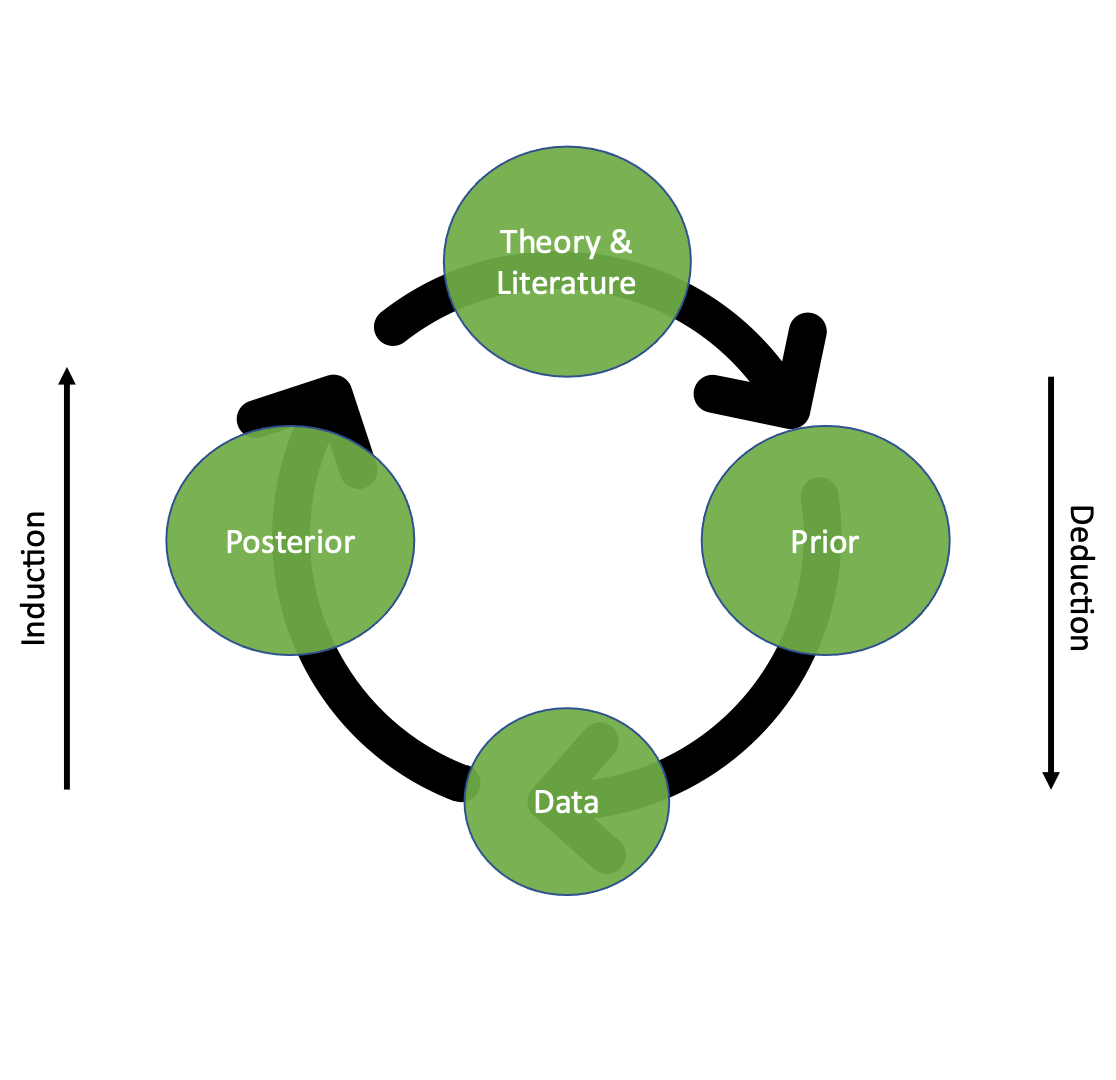
\includegraphics[width = .65\paperwidth]{learning.png}
\caption{The Bayesian learning cycle is a reasoning framework that allows scientists, citizens, and learners to integrate the strengths of inductive and deductive reasoning while making sense of data in light of prior beliefs.}
\label{fig:The Bayesian Learning Cycle}
\end{center}
\end{figure*}
Having introduced Bayes Theorem and an application of Bayes Theorem as a cycle through which individuals can learn, we show how Bayes Theorem can be used to demonstrate several principles that are relevant to building trust in science.

\section{The Epistemological Principles that Follow from Bayes Theorem}

In the previous section, we emphasized the idea that hypotheses, or ideas, gain credibility when they predict the data well, and lose credibility when they predict new data poorly \parencite{WagenmakersEtAl2016CD}. This idea generalizes to the ``Fundamental Inductive Pattern'':
\begin{quotation}
``This inductive pattern says nothing surprising. On the contrary, it expresses a belief which no reasonable person seems to doubt: \emph{The verification of a consequence renders a conjecture more credible}. With a little attention, we can observe countless reasonings in everyday life, in the law courts, in science, etc., which appear to confirm to our pattern.'' \parencite[pp. 4-5]{Polya1954Vol2}
\end{quotation}

The rule from Equation~\ref{eq:BayesRule} includes the constant term $p(\text{data})$, which does not involve $\theta$. As a result, Bayes' rule can be re-written as:
\begin{equation}
\label{eq:BayesRulePropto}
p(\theta \mid \text{data}) \propto p(\text{data} \mid \theta) \times p(\theta),
\end{equation}
where `$\propto$' stands for `is proportional to'. Thus, Bayes' rule states that our posterior knowledge $p(\theta \given \text{data})$ is proportional to the likelihood $p(\text{data} \given \theta)$ (or the extent to which the observed data are expected given $\theta$) multiplied by our prior knowledge $p(\theta)$.

Equation~\ref{eq:BayesRulePropto} emphasizes that the posterior uncertainty about $\theta$ is a \emph{compromise} between our prior uncertainty about $\theta$ and the predictive performance of $\theta$. But, the posterior uncertainty after having observed the first datum becomes the prior uncertainty for the next datum---and any other data (cf. Figure~\ref{fig:WindowsMacSequential}). Consequently, after having observed another datum, the posterior uncertainty represents a compromise of a compromise. As the data accumulate, the posterior uncertainty is more and more determined by predictive performance, and the impact of the initial uncertainty about $\theta$ is increasingly watered down: `the data overwhelm the prior' \parencite{WrinchJeffreys1919}.

This implies (but does not dictate, as we discuss next) that a constant stream of accumulating data ought to bring any two people into an arbitrarily close agreement, no matter how divergent their opinions may have been at the outset. There are two important caveats here. 

First and foremost, the data only overwhelm the prior if that prior is neither equal to zero (denoting an impossibility) nor one (denoting absolute certainty). If someone already knows for certain that a hypothesis is true or false, then you cannot adjust your opinion in light of the data: your initial opinion will be your final opinion, no matter what the data may indicate. Philosophically, adopting such priors is a dangerous practice; for instance, in antiquity the adage of the \emph{New Academy} --a school of skeptics headed by Carneades-- was ``never assert absolutely''. In modern times, Lindley popularized this idea in statistics and coined it ``Cromwell's rule'' \parencite[p. 104]{Lindley1985}.

The second caveat is that, in real life, the data are sometimes relatively slow to overwhelm the prior, as people can be reluctant to change their beliefs (for a Bayesian model see \cite{Gershman2019}). A more extreme case is \emph{belief polarization}: confronted with the same stream of information, two people who hold different opinions may drift further apart instead of moving closer together (but see \cite{Anglin2019}). This appears irrational, but several Bayesian accounts have been offered to explain the phenomenon (e.g., \cite{CookLewandowsky2016,JernEtAl2014}).

Next, consider two specific values for $\theta$, $\theta_1$ and $\theta_2$. We can use Bayes' rule to obtain the posterior probability for each one:
\begin{align}
p(\theta_1 \mid \text{data})& =  \frac{p(\text{data} \mid \theta_1) \times p(\theta_1)}{p(\text{data})}\\
p(\theta_2 \mid \text{data})& =  \frac{p(\text{data} \mid \theta_2) \times p(\theta_2)}{p(\text{data})}.
\end{align}
When we divide the posterior probabilities the common term, $p(\text{data})$, drop out, and we have:
\begin{equation}
    \frac{p(\theta_1 \mid \text{data})}{p(\theta_2 \mid \text{data})} = \frac{p(\theta_1)}{p(\theta_2)} \, \times \, \frac{p(\text{data} \mid \theta_1)}{p(\text{data} \mid \theta_2)}.
\end{equation}
We replace $\theta_2$ with $\mathcal{H}_1$ (i.e., the alternative hypothesis, in which a test-relevant parameter $\xi$ is free to vary) and $\theta_1$ with $\mathcal{H}_0$ (i.e., the null hypothesis in which $\xi$ takes on a fixed value, for instance $\xi=0$):
\begin{equation}
    \frac{p(\mathcal{H}_1 \mid \text{data})}{p(\mathcal{H}_0 \mid \text{data})} = \frac{p(\mathcal{H}_1)}{p(\mathcal{H}_0)} \, \times \, \frac{p(\text{data} \mid \mathcal{H}_1)}{p(\text{data} \mid \mathcal{H}_0)}.
\end{equation}
This way of writing Bayes' rule highlights that extraordinary claims require extraordinary evidence -- if a particular hypothesis $\mathcal{H}_1$ is extremely unlikely a priori, the prior odds $\frac{p(\mathcal{H}_1)}{p(\mathcal{H}_0)}$ are stacked against it, and for the posterior odds to favor $\mathcal{H}_1$ the support from the data (i.e, the degree to which $\mathcal{H}_1$ predicts $\mathcal{H}_0$) needs to be overwhelmingly strong.   

Bayes' rule can also be shown to embody the \emph{principle of parsimony}: the rule implicitly contains a preference for the simplest model that explains the data well. To see this, consider a coin with two sides and let parameter $\xi$ indicate the chance that the coin lands heads on any throw. The null hypothesis holds that the coin is fair, with heads and tails equally likely: $\mathcal{H}_0: \xi = \nicefrac{1}{2}$. The alternative hypothesis that we entertain here specifies that the coin may be any of the following options with equivalent likelihood: double-tails, fair, or double-heads, $\mathcal{H}_1: \xi \in \{0, \nicefrac{1}{2}, 1\}$.

The coin is tossed and heads is observed. The probability of this datum is \nicefrac{1}{2} under $\mathcal{H}_0$; under $\mathcal{H}_1$, it is $p(\text{heads} \given \xi=0) \cdot p(\xi=0 \given \mathcal{H}_1) + p(\text{heads} \given \xi=\nicefrac{1}{2}) \cdot p(\xi=\nicefrac{1}{2} \given \mathcal{H}_1) + p(\text{heads} \given \xi=1) \cdot p(\xi=1 \given \mathcal{H}_1) = 0 \cdot \nicefrac{1}{3}  + \nicefrac{1}{2} \cdot \nicefrac{1}{3} + 1 \cdot \nicefrac{1}{3} = \nicefrac{1}{2}$. So, the datum is equally likely under $\mathcal{H}_0$ and $\mathcal{H}_1$: both models receive an equal amount of support. This means the first outcome does not change our conviction concerning $\mathcal{H}_0$ versus $\mathcal{H}_1$. The datum did, however, change our beliefs about $\xi$ under $\mathcal{H}_1$. Specifically, we now know that $\xi$ cannot be zero; moreover, the datum was twice as likely under $\xi=1$ as under $\xi = \nicefrac{1}{2}$, so that our posterior distribution for $\xi$ under $\mathcal{H}_1$ is now $p(\xi = \nicefrac{1}{2}) = \nicefrac{1}{3}, p(\xi = 1) = \nicefrac{2}{3}$. 

The coin is tossed a second time and it lands tails. Under $\mathcal{H}_0$, the probability of this happening is again $\nicefrac{1}{2}$, so the total probability for the data sequence $\{\text{heads}, \text{tails}\}$ under $\mathcal{H}_0$ equals $\nicefrac{1}{2} \cdot \nicefrac{1}{2} = \nicefrac{1}{4}$. Under $\mathcal{H}_1$, the probability of the second toss landing heads is computed under the posterior distribution obtained after the first toss, and this yields: $p(\text{tails} \given \xi = \nicefrac{1}{2}) \cdot p(\xi=\nicefrac{1}{2} \given \mathcal{H}_1) + p(\text{tails} \given \xi = 1) \cdot p(\xi=1 \given \mathcal{H}_1) = \nicefrac{1}{2} \cdot \nicefrac{1}{3} + 0 \cdot \nicefrac{2}{3} = \nicefrac{1}{6}$. The total probability for the data sequence $\{\text{heads}, \text{tails}\}$ under $\mathcal{H}_1$ equals $\nicefrac{1}{2} \cdot \nicefrac{1}{6} = \nicefrac{1}{12}$. This means that the observed data provided $(\nicefrac{1}{4}) / (\nicefrac{1}{12}) = 3$ times more support for $\mathcal{H}_0$ than for $\mathcal{H}_1$. This happens because $\mathcal{H}_1$ "spreads out" its predictions, hedging its bets. In contrast, the simple model $\mathcal{H}_0$ made a precise prediction. 

Instead of learning about the predictive performance one observation at a time of $\mathcal{H}_0$ and $\mathcal{H}_1$, we could also have considered the probability that the models assign to the entire sequence $\{\text{heads}, \text{tails}\}$. Under $\mathcal{H}_0$ we again have $\nicefrac{1}{2} \cdot \nicefrac{1}{2} = \nicefrac{1}{4}$. Under $\mathcal{H}_1$, we notice that the data falsify both $\xi=0$ and $\xi=1$. This leaves $\xi=\nicefrac{1}{2}$, which suggests the same answer as under $\mathcal{H}_0$, that is $\nicefrac{1}{2} \cdot \nicefrac{1}{2} = \nicefrac{1}{4}$. However, we need to multiply this probability with $\nicefrac{1}{3}$, the prior probability that $\xi=\nicefrac{1}{2}$. This is the penalty for complexity that $\mathcal{H}_1$ pays for entertaining three different values of $\xi$ from the outset. Thus, in addition to reflecting the principle of parsimony and highlighting the utility of parsimonious explanations, Bayes rule includes a automatic ``Ockham's razor'' \parencite{Jeffreys1939,JefferysBerger1992} in the sense that daring predictions are rewarded when they come true.

Finally, we can also write Bayes' rule as follows:
\begin{equation}
\begin{split}
    p(\mathcal{H}_1 \mid \text{data})& = \frac{p(\text{data} \mid \mathcal{H}_1) p(\mathcal{H}_1)}{p(\text{data})}\\
    & = \frac{p(\text{data} \mid \mathcal{H}_1) p(\mathcal{H}_1)}{p(\text{data} \mid \mathcal{H}_1) p(\mathcal{H}_1) + p(\text{data} \mid \mathcal{H}_0) p(\mathcal{H}_0)}.
\end{split}
\end{equation}
This equation shows that the posterior plausibility is dictated by the predictive performance for $\mathcal{H}_1$ and $\mathcal{H}_0$, weighted by the prior plausibility of each hypothesis. In other words, ``The Bayesian world is a comparative world in which there are no absolutes.'' \parencite[p. 308]{Lindley2000}. This is in stark contrast to $p$-value statistical hypothesis testing, in which a statistical model (the null hypothesis) is judged in isolation. 
Having introduced Bayes Theorem and some principles that may follow from it, we next make the case how Bayes could support science literacy at large before delving into implications for science teaching and learning.

\section{A Bayesian Perspective and Science Literacy}

We conceive that Bayesian methods can enhance science literacy or a range of capabilities that people may possess which have value (individually or collectively) to them \parencite{council2016science}. These capabilities range from core \ital{literacies}, including numeracy and textual literacy (what is mostly thought of in common parlance concerning literacy), content knowledge, and epistemic knowledge \parencite{council2016science}. A potentially powerful way in which Bayesian ideas can inform discussions of science literacy is to provide individuals with a principle for combining their prior understanding with new evidence. Along this line, Bayes and the Bayesian Learning Cycle can provide a tool for people (and learners) to combine their understanding with new evidence (and data) rigorously and coherently.

A timely example can help to illustrate how a Bayesian perspective on a topic relevant to science literacy may offer a different way forward. Consider a salient topic, medical vaccines for diseases, such as Polio and the disease caused by the coronavirus SARS-CoV-2, COVID-19. Most evidence suggests that vaccines have been safe, historically, and are generally safe, at present (Centers for Disease Control and Prevention, 2021). Nevertheless, they are not perfectly safe, as unlikely, adverse outcomes do happen, and there may be adverse side effects from some vaccines that research has not yet revealed. In light of this evidence, consider the development of a new vaccine, such as those available at the time of this writing for COVID-19. Some use long-established methods of vaccine development (namely, deactivating SARS-CoV-2 particles but retaining cell signaling proteins to which humans develop an immune response—and, after, a degree of immunity) and injecting these deactivated virus particles into people), whereas others use a new mechanism (namely, injecting messenger RNA into people; this messenger RNA is then transcribed by cells in people’s bodies to produce a particular protein common to SARS-CoV-2 particles, which human’s bodies then learn to recognize to develop immunity.  

How should we consider evidence about the vaccines? Before any data from medical clinical trials, it would be reasonable to consider these vaccines to probably be safe in light of the safety of other vaccines (and based on similarities in their mechanisms of action), but to have a strong degree of caution about how safe they are. After initial trials were completed, the degree of safety that individuals associate with these vaccines—in light of the prior and the limited evidence—could increase, but still not be near the level of safety that many would consider acceptable. Following the completion of clinical trials that show minimal side effects (holding aside their efficacy), one’s estimates of the safety of these vaccines could increase by a substantial amount, but concerns could remain, particularly for messenger RNA vaccines, which are newer, and may, plausibly, have unintended side effects.

While the complex weighting of the evidence above may seem natural to a scientist, it is challenging for many. In the following, we showcase how several important insights for weighting evidence follow directly from Bayes' rule. Thus, we argue that emphasizing Bayesian reasoning can support science literacy by providing people with a principled way to weighting evidence that is accessible because it builds on peoples' prior ideas.

In the context of the above example on SARS-CoV-2, the result of applying Bayes Theorem in a heuristic mode is a non-binary inference, one that doesn't speak to whether or not the vaccine is safe, but to what degree it is safe, doing so with a language of probability and uncertainty. Though a small difference, discussing the safety of vaccines on these terms can provide a more solid foundation for principled disagreements and arguments. In addition, Bayes provides a heuristic and a language for engaging with uncertainty in a science literacy context in a principled way that is in line with how most of us likely already interpret data \parencite{tgk06, gw12, gh95}; A Bayesian perspective can provide people with a way to talk about weighing between ideas and their prior beliefs and new information and data. In short, Bayes gives people a chance to deal with uncertainty in a principled but accessible manner.

In addition, many themes introduced in the section on the epistemological principles that follow from Bayes Theorem are relevant to the aim of supporting science literacy. First, \ital{even individuals with different initial beliefs may be brought closer to an agreement in light of data} that serves as evidence for a particular belief or hypothesis. In this way, Bayes Theorem illustrates--at the conceptual level as well as statistically--how individuals may be unlikely to agree based on the limited or weak information, but that this can shift in light of accumulating data. As we noted earlier, this is far from a deterministic process, and \ital{holding initial beliefs that a hypothesis has a probability of zero or one means that data does not affect one's beliefs}. This suggests that a cultural norm and principle for science literacy can be to always reserve a degree of uncertainty such that one could be influenced by (new) data or evidence: From a Bayesian perspective, \ital{our knowledge is uncertain and open to change and revision} so long as we remain open to new evidence.

Related to the importance of not holding scientific beliefs with a probability of zero or one, another principle that follows from Bayes Theorem is that \ital{extraordinary claims require extraordinary evidence}, and that unlikely or implausible hypotheses or claims are likely to necessitate strong empirical data to be convincing to others. A corollary of this principle is that we should strong initial or prior beliefs can serve as a tool through which we can discuss extraordinary claims: Except in light of strong evidence, "ordinary" claims can serve as the default for citizens and scientists making sense of unusual and potentially biased claims. Similarly, Bayes Theorem demonstrates that the \ital{simplest possible explanation--the most parsimonious explanation--is often the best explanation}. 

In sum, a Bayesian perspective offers a general approach to science literacy that can account for uncertainty in a rigorous and principled manner. In addition, a number of principles that follow from Bayes Theorem, such as being receptive to new evidence and weighting that evidence per its strength in light of the strength of one's initial beliefs or understanding could bolster science literacy---and how the public comes to understand and gain trust in science.

\section{A Bayesian Perspective and Science Education}

Research on the role of Bayes in science education has mostly been carried out in the context of undergraduate statistics education, in which there have been several calls to action \parencite{gpkpwc18, h_a20}, examples and design options \parencite{a02, b02,g08, w17, h_j20} and debate \parencite{jrhrr20} over how to advance the place of Bayesian methods in undergraduate statistics and data science degree programs. The accessibility of Bayesian methods in undergraduate classes is the result of advances in the necessary (for many uses) computer power \parencite{gpkpwc18} as well as the availability of tools that facilitate Bayesian analysis, especially for newcomers \parencite{ah20}. As evidenced by the recent special issue of the \emph{Journal of Statistics Education} of which several of the above-referenced articles are part, the pedagogy of Bayesian statistics is an active area of research in statistics education at the undergraduate level.

There is little research outside of statistics education in the broader science education community. Two publications merit mention though. The work of \textcite{so12} and \textcite{n11} both applied Bayesian perspectives to the science practice of argumentation. Szu and Osborne presented the case for how and why Bayes Theorem can apply to research and practice on scientific reasoning, broadly, and argumentation, particularly. This paper represents the most comprehensive account of the relevance of Bayesian methods for science education. Szu and Osborne argue that Bayes is useful as both a formal mathematical tool and a conceptual one; indeed, they write that considering the degrees of certainty in beliefs that individual students hold—different from applications of Bayes Theorem that follow more or less deterministically from ``external, objectively probabilistic systems'' (p. 61)—is ``the key leap that characterizes the debate about the value of Bayesian inference as a model of scientific reasoning'' (p. 61). In this way, Szu and Osborne argue that the greatest use of Bayes Theorem in science classrooms is as a model of informal scientific reasoning, aligning with similar (informal) approaches to inference within the statistics education research community \parencite{batanero2016research, mr18}. They offer some research-related backing for the use of Bayes Theorem (e.g., noting how conceptual change research, particularly, and constructivist research, broadly, can both be explained coherently within a Bayesian approach) as well as some practical, instructional recommendations, some of which we detail later in this section.

\textcite{n11} work on Bayesian approaches to argumentation complement the work of Szu and Osborne in that Nussbaum describes both an application of Bayesian methods in K-12 classroom contexts and ideas about how Bayesian methods can serve as an analytic framework for students’ argumentation. Concerning the latter, Nussbaum describes how the social issue of raising taxes to provide resources to homeless individuals was a rich context for students to engage in forms of Bayesian reasoning. In this application, Nussbaum describes how the prior and likelihood could be obtained from empirical evidence—in this way, illustrating what \textcite{so12} characterize as the more externally objective use of Bayes Theorem—and how the estimates that result from applying Bayes Theorem led students to re-evaluate their initial arguments. 

In summary, the work of \textcite{so12} and \textcite{n11} begin to apply Bayesian ideas to science education and other relevant classroom contexts, making Bayesian ideas more vivid in the process. Curiously, no work has applied Bayesian methods to another science practice, that of analyzing and interpreting data; one for which Bayesian methods have clear conceptual applicability and utility, but one for which the absence of suitable tools may provide to be a barrier. In this way, Bayesian methods could serve as a cross-cutting concept \parencite{nrc12} that unites the practice of argumentation with analyzing and interpreting data and using mathematics and computational thinking.

Bayesian methods have some utility in science education, even if that utility is under-realized at present. Next, we present some of the specific ways Bayesian methods could enhance science education—and could do so in a way that makes Bayes more tractable.

First, curricular resources and pedagogical approaches that take a Bayesian perspective can be developed. These could elaborate on the ideas of \textcite{so12} and \textcite{n11}. At a high-level, Szu and Osborne write that to reason about data in light of their initial beliefs (and to construct a kind of informal likelihood statistic), students “need to see judgments about data and evidence being an assessment not only of the probability of the hypothesis being correct but also of it being wrong” (p. 67). Filling in more details, speaking from both the perspective of a researcher (of argumentation) and an educator (or, a designer of classroom activities), Nussbaum summarizes that using Bayes “forces one to (a) think about an issue from different perspectives, (b) reflect on one’s range of certainty and uncertainty and (c) conduct a simple computer simulation (e.g., calculating the product) that integrates various facets of the issue together and affords further reflection” (p. 99). 

The work of \textcite{so12} and \textcite{n11} can be complemented by finer-grained instructional techniques, especially those advanced by statistics educators to support students to reason about uncertainty probabilistically. A benefit of these strategies is that they can help to address some of the ingrained challenges that people and learners face when attempting to reason probabilistically \parencite[e.g., ][]{tk74}. Particularly, \textcite{bkbm18} for instance, suggest replacing probabilities with natural frequencies. This suggestion is in alignment with prior work by \textcite{gh95} on how different representations of probabilities can explain some of the challenges that people and learners face. In addition, \textcite{me14}—building on much earlier experimental work by \textcite{wason1971natural}—provide a simple example of how even fourth-graders, with the right tools to represent probabilities, can support students to transition from logical to probabilistic reasoning. These could also support the aim of developing unplugged versions of Bayesian analyses. 

Science education researchers may consider how teachers can support students to reason about uncertainty in a way that aligns with a Bayesian perspective. While some scholars have contributed foundational work demonstrating how this uncertainty can be productive as a part of teaching practice \parencite{manz2018supporting}, a broad and formal perspective on how uncertainty can be approached in science education is needed. Further, a better understanding of uncertainty can help to learn about scientific--and other--concepts where probability plays a key role; it may be that learning about how Bayes rule can be used in legal or medical contexts could impress upon students the cross-cutting nature of probability and uncertainty.  

Finally, recently developed tools, particularly the JASP statistical software \parencite{JASP2020}, may be helpful. JASP allows for both conventional frequentist as well as Bayesian versions of commonly used statistical tests, such as t-tests and regression analyses. There are many accessible guides available for specifying Bayesian versions of analyses \parencite{v20, wagenmakers2018bayesian}, and there is a great potential in building particular examples within JASP (that are aligned to science education curricular standards) that could support science educators to have greater access to the power of Bayesian methods in their classrooms. Another possibly useful tool could be Bayesian networks (see Bayes Box; Bayes Box, 2021), which could be used to model complex systems in a way that is similar to other tools used in science education for modeling complex systems, such as \textcite{20}.

\section{Conclusion}

In summary--to this point--we have introduced Bayes as a powerful way of conceptualizing probability and uncertainty. These are two concepts that are ubiquitous in the learning, doing, and communicating of science and therefore critical aspects of science literacy. However, probability and uncertainty are also infamously challenging concepts—for experts and laypersons alike \parencite{gkv04, s07, tk74}. Thus, it is not surprising when the public misinterprets statements about probability and uncertainty but the consequences may be dire when trust in science is eroded, and, sadly, examples of this are plentiful during current the COVID-19, e.g., the efficiency of masks in preventing the spread of COVID and the efficiency of the AstraZeneca vaccine were strongly questioned, delaying efforts to combat the pandemic. The public, however, can hardly be blamed for this in light of the prevalent findings that the frequentist conceptualizations of probability and uncertainty in school are challenging and uncommonly align with or build on peoples’ intuitions. As research from cognitive and psychological science as well as emerging work from statistics and statistics data science education demonstrates, conceptualizing probability and uncertainty from a Bayesian perspective better aligns with peoples’ intuitions \parencite{kl18, so12} about these concepts and thus has the potential to support learning about probability and uncertainty in science. Moreover, a Bayesian perspective is unique in that it is akin to a cross-cutting concept in the sense of a style of reasoning \parencite{so12, ork18} that blends conceptual ideas with practices: Bayes is both a philosophical and psychological perspective on how to learn from data as well as a statistical framework. Indeed, a key potential benefit of Bayes may be that it provides a framework for helping students to transition from their conceptual understanding of scientific ideas to quantitatively analyzing data.  

Even at a time in which science has made and continues to make great advances, the history of science suggests that uncertainty will not be removed (or even reduced) given scientific progress \parencite{fara2010science}; looking ahead, being able to effectively navigate, counsel, and act in the midst of uncertainty may be as important as it has been at other uncertain points in history. Like the surprising utility of a Bayesian perspective in domains that are similar to education (e.g., developmental science), might an unexpected feature of a Bayesian perspective be that embracing uncertainty--equipped with the tools that Bayesian methods provide--makes individuals and societies more confident? In short, can we build trust in science by embracing uncertainty? We think that these are questions that are \ital{likely} to yield positive results for science educators and those advocating for a more rationale and scientific citizenry and for science learners.

\printbibliography

\end{document}
